\vspace{-5pt}
\subsubsection{Graph-based Metrics}
\begin{wrapfigure}{r}{0.32\textwidth}

    \centering
    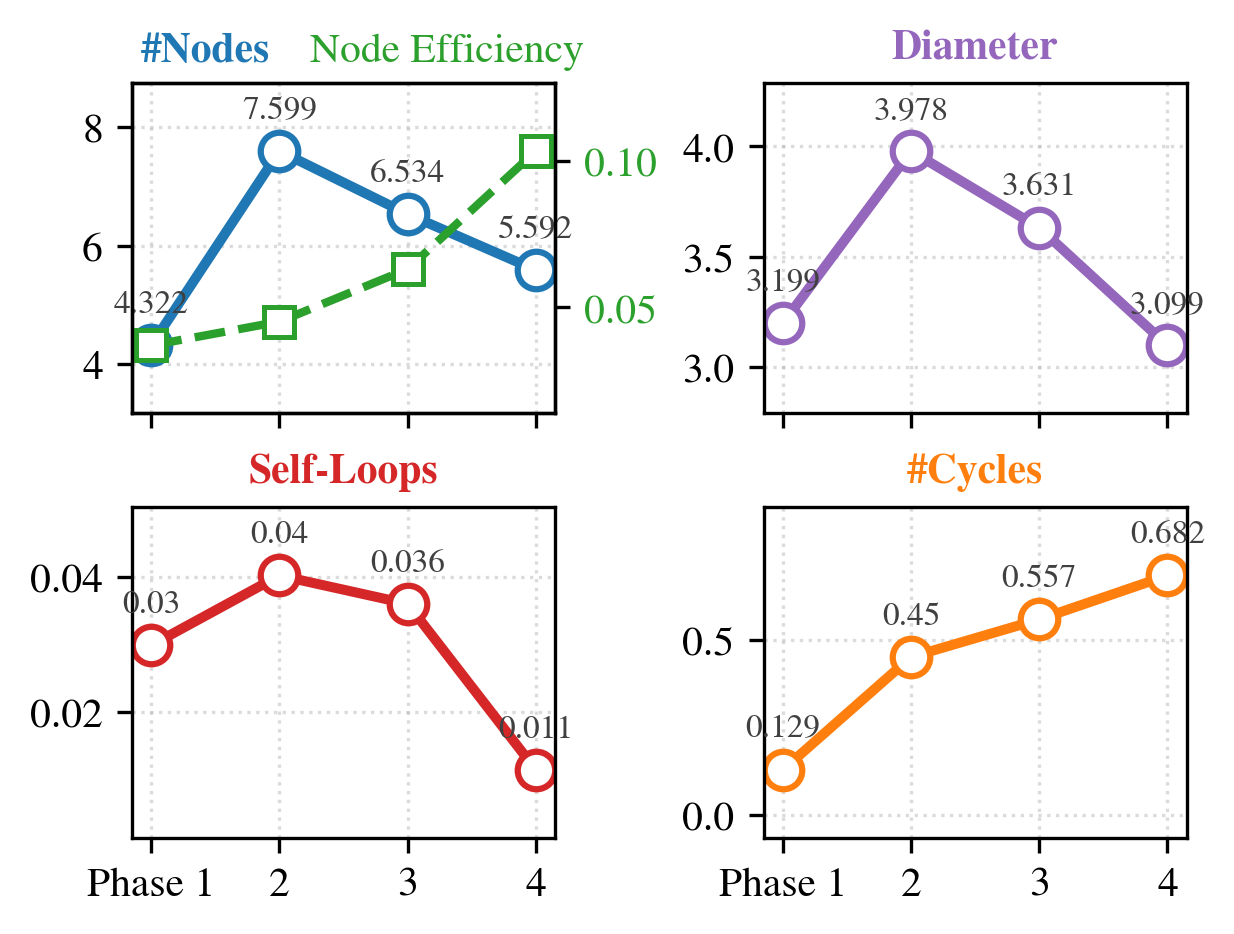
\includegraphics[width=\linewidth, height=3.3cm, keepaspectratio]{figures/nodesefficiency.png}
% 
    \captionof{figure}{Graph metrics}

    \label{fig:graph_metrics}
\end{wrapfigure} 
\vspace{-5pt}
To systematically characterize the topology evolution of \hero, we model each trajectory as a graph $\mathcal{G}_{\tau}=(V, E)$ where nodes represent agents and edges denote interactions. We quantify structural and functional properties via defining graph-theoretic metrics:
\textbf{(a) Number of agents $|V|$}: the total distinct agents involved in a trajectory, reflecting the breadth of collaboration.
\textbf{(b) Node efficiency}: per-agent contribution, formally by $\frac{\text{F1}(\tau)}{|V|}$, capturing per-agent utility.
\textbf{(c) Self-Loops}: the frequency of self-transitions, reflecting potential redundancy or degenerate reasoning.
\textbf{(d) Number of cycles}: count of closed-loop paths capturing iterative reasoning patterns.
\textbf{(e) Diameter}: longest shortest-path between any two nodes, representing maximum reasoning depth. 

We segment learning into four phases - initial, exploration, refinement, and optimization, and analyze normalized metrics per question type. As shown in Fig.~\ref{fig:graph_metrics}, Early trajectories are narrow and shallow, with low agent counts, minimal cycles, and limited diameter, reflecting sparse coordination. During exploration, the system dynamically recruits more agents, increasing diameter and cycle formation, capturing iterative reasoning and intermediate verification. By the refinement phase, trajectories contract: redundant agents and self-loops are pruned, diameter decreases, and node efficiency rises. This selective retention is guided by the experience library, which reinforces high-value interaction topologies, and by prompt evolution, which refines agent behaviors and intermediate outputs. The optimized phase exhibits compact chains with minimal nodes, high per-agent utility, and strategically preserved cycles, representing a balance of efficiency and robustness.

Overall, the evolving topologies reveal that \hero’s dual mechanisms - structured experience retrieval and adaptive prompt evolution enable a principled transition from exploratory, diffuse agent interactions to compact, high-utility, and resilient multi-agent system.